\clearpage
\section{Lösungskonzept}\label{sec:Loesungskonzept}
In Abbildung \ref{img:Grobkonzept} ist das Blockschaltbild ersichtlich, welches alle Teilsysteme und Einheiten darstellt. Es ist modular gegliedert und bietet eine Übersicht der Schnittstellen zwischen den einzelnen Modulen. 

Das Lösungskonzept selbst gliedert sich in drei physikalisch getrennte Einheiten. Das \textit{Machine Controll System} (MCS), das \textit{Human Maschine System} (HMS) und den Drucker selbst, einen \textit{Ender 3} der Firma \textit{Creality3D}. 

Das MCS bildet den Hauptbestandteil des Lösungskonzepts. Es beinhaltet die Druckersteuerung und die Kommunikationsschnittstellen. Um diese zwei Aufgaben zu separieren befinden sich zwei Mikroprozessoren in dieser Einheit. Zusätzlich werden die Aktoren und Sensoren des 3D-Druckers  angesteuert und eingelesen. Eine Statusanzeige zur Visualisierung des Zustandes ist ebenfalls angedacht.

Das HMS bildet die Benutzerschnittstelle über ein internetfähiges Gerät. Es kommuniziert mittels WLAN mit dem MCS. Über dieses Gerät können Druckaufträge verwaltet und überwacht werden. Auf dem 3D-Drucker befinden sich alle Aktoren und Sensoren. Sie werden über Kabelverbindungen an das MCS angebunden.



\begin{figure}
	\centering
	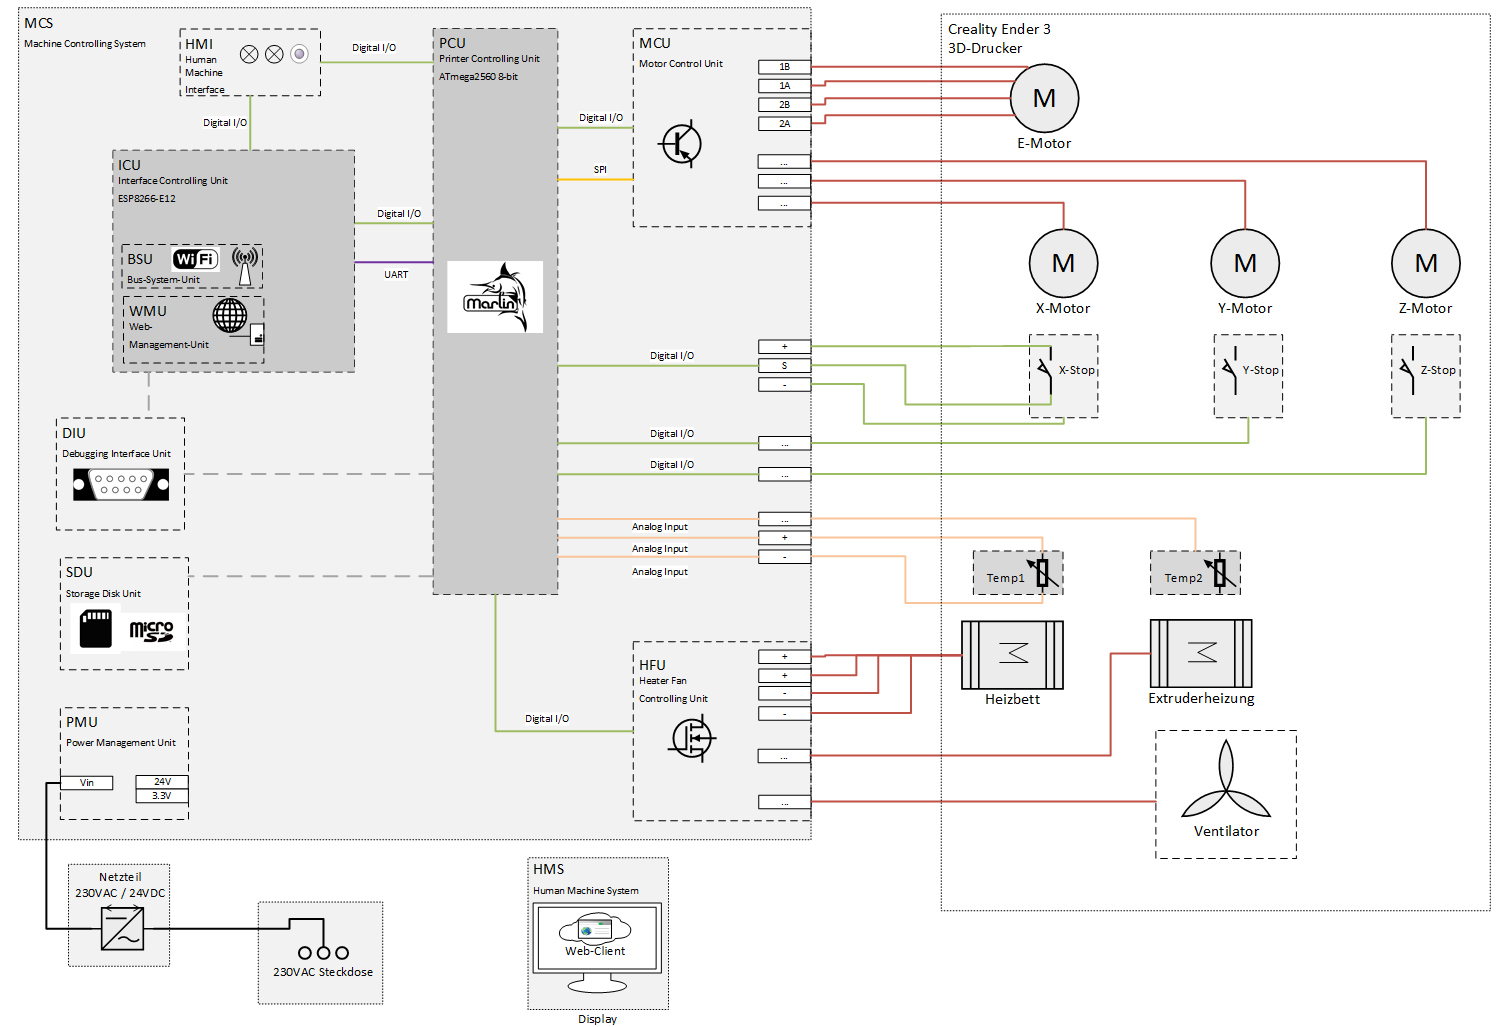
\includegraphics[scale=0.58,angle=90]{19FS-pro4E-Team1_Grobkonzept_25022019_ohne_Rahmen.png}
	\caption{Blockschaltbild des Lösungskonzepts}
	\label{img:Grobkonzept}
\end{figure} 








